\documentclass[../DS08.tex]{subfiles}%
\graphicspath{{./figures/}}%

% \subimport{/home/nora/Documents/Enseignement/Prepa/bpep/exercices/DS/Chimie_de_l_azote/}{sujet.tex}%

\begin{document}%

\section[91]"P"{Propriétés de l'azote\ifcorrige{~\small\textit{(D'après banque PT
		2008)}}}

\enonce{%
	\begin{center}
		\begin{framed}
			\large\bfseries
			Les parties sont indépendantes
		\end{framed}
	\end{center}

	\begin{tcn}[sidebyside](data){Données à \SI{25}{\degreeCelsius}}
		\begin{itemize}
			\item $\pk(\ce{{HNO_3}_{\aqu}/{NO_3}^-_{\aqu}}) = \num{-1.37}$
			\item $\pk(\ce{{HNO_2}_{\aqu}/{NO_2}^-_{\aqu}}) = \num{3.3}$
			\item $\pk(\ce{{NH_4}^+_{\aqu}/{NH_3}_{\aqu}}) = \num{9.2}$
			\item $M(\ce{Cu}) = \SI{63.5}{g.mol^{-1}}$
			\item $M(\ce{Ti}) = \SI{48.0}{g.mol^{-1}}$
			\item $M(\ce{N}) = \SI{14.0}{g.mol^{-1}}$
			\item $M(\ce{NO3^-}) = \SI{62.0}{g.mol^{-1}}$
			\item $R = \SI{8.314}{J.K^{-1}.mol^{-1}}$
		\end{itemize}
		\tcblower
		\begin{itemize}
			\item $E^\circ(\ce{{NO_3}^-_{\aqu}/{HNO_2}_{\aqu}}) = \SI{0.94}{V}$
			\item $E^\circ(\ce{{NO_3}^-_{\aqu}/{NO}_{\gaz}}) = \SI{0.96}{V}$
			\item $E^\circ(\ce{{HNO_2}_{\aqu}/{NO}_{\gaz}}) = \SI{0.99}{V}$
			\item $E^\circ(\ce{{Cu}^{2+}_{\aqu}/{Cu}_{\sol}}) = \SI{0.34}{V}$
			\item $E^\circ(\ce{{Fe}^{3+}_{\aqu}/{Fe}^{2+}_{\aqu}}) = \SI{0.77}{V}$
			\item $E^\circ(\ce{{MnO_4}^-_{\aqu}/{Mn}^{20}_{\aqu}}) = \SI{1.5}{V}$
			\item Volume molaire gaz parfait $V_m = \SI{22.4}{L.mol^{-1}}$
			\item $\Fc = \SI{9.65e4}{C.mol^{-1}}$
		\end{itemize}
	\end{tcn}
}%

\subsection{$\mathllap{\textcolor{Red}{/18}\hspace*{1.5cm}}$Synthèse de l'ammoniac}%

\enonce{%
	Le procédé \emph{Haber} est un procédé chimique en phase gazeuse servant à la
	synthèse de l'ammoniac \ce{NH3_{\gaz}} par hydrogénation du diazote
	\ce{N2_{\gaz}} atmosphérique par le dihydrogène \ce{H2_{\gaz}} en présence
	d'un catalyseur.
}%

\QR[2]{%
	Écrire l'équation de la réaction, notée (1) pour une mole de diazote.
}{%
	\leavevmode\vspace*{-15pt}\relax
	\begin{gather*}
		\ce{3{H_2}_{\gaz} + {N_2}_{\gaz} \stm{\stm(un){=}} 2 {NH_3}_{\gaz}}
		\tag{1}
	\end{gather*}
}%

\QR[4]{%
	Exprimer le quotient de réaction $Q_r$ associé à l'équilibre (1) en fonction
	des activités d'abord, puis des quantités de matière de chaque constituant
	présent dans le système, de la quantité de matière totale $n\ind{tot}$, de la
	pression $P$ du système et de la pression standard $P^\circ = \SI{1}{\bar}$.
}{%
	\label{Qr}
	\leavevmode\vspace*{-15pt}\relax
	\begin{gather*}
		Q_r \stm{=} \dfrac{a(\ce{NH3})^2}{a(\ce{H2})^3 a(\ce{N2})}
		\Lra
		Q_r \stm{=}
		\dfrac{n_{\ce{NH3}}^2n\ind{tot}^2 (P^\circ)^2}{n_{\ce{H2}}^3 n_{\ce{N2}} P^2}%
	\end{gather*}
	On rappelle que pour le constituant gazeux \ce{X_i}, l'activité s'écrit $a_i
		\stm{=} \cfrac{p_i}{P^\circ} \stm{=} \cfrac{n_i P}{n\ind{tot} P^\circ} $ avec
	$p_i$ la pression partielle de \ce{X_i} et $n_i$ sa quantité de matière.
}%

\QR[2]{%
	Indiquer à quoi est égal le quotient de réaction lorsque le système atteint
	l'équilibre chimique. On n'attend pas de valeur numérique. Comment s'appelle
	cette loi~?
}{%
	À l'équilibre, le quotient de réaction est \xul{égal à la constante
		d'équilibre $K^\circ$} \pt{1}. C'est la loi \xul{d'action de masse} \pt{1}, ou
	de \textsc{Guldberg-Waage}
}%


\QR[2]{%
	On suppose que le système a atteint son état d'équilibre. Sans modifier la
	composition du système et en conservant la température constante, on élève la
	pression $P$. Dans quel sens évolue l'équilibre (1)~?
}{%
	D'après l'expression obtenue question \ref{Qr}, une élévation de pression sans
	modifier la composition du système diminue \pt{1} le quotient de réaction. Le
	système va donc évoluer dans le \xul{sens direct} \pt{1} (formation du
	produit \ce{NH3}) pour retourner à l'équilibre.
}%


\QR[1]{%
	Indiquer l'intérêt d'utiliser un catalyseur dans la synthèse de l'ammoniac.
}{%
	Un catalyseur permet \xul{d'augmenter la vitesse de réaction}. \pt{1}
}%

\QR[7]{%
	La synthèse de l'acide nitrique \ce{HNO3} à partir de l'ammoniac passe
	notamment par les intermédiaires \ce{NO} et \ce{NO2}. Proposer une
	représentation de Lewis de \ce{NH3}, \ce{NO2} et \ce{HNO3} sachant qu'aucune
	d'entre elles ne fait intervenir de liaison \ce{O-O} et qu'une de ces
	représentations ne respecte pas la règle de l'octet.
}{%
	\leavevmode\vspace*{-15pt}\relax
	\begin{tasks}[label=\bdmd](3)
		\task Hydrogène~: 1 électron de valence
		\task Azote~: 5 éle\stk(un){c}trons de valence
		\task Oxygène~: 6 électrons de valence
	\end{tasks}
	\vspace{-15pt}
	\noindent
	\begin{minipage}[t]{.30\linewidth}
		\begin{gather*}
			\fatbox{\textbf{\ce{NH3}}}
			\\
			n\ind{é,tot} = 8
			\stm{\Lra}
			\text{4 doublets}
			\\[1em]
			\cfig{
				H-\charge{90=\|,-45:10pt={\pt{1}}}{N}(-[-90]H)-H
			}
		\end{gather*}
	\end{minipage}
	\hfill
	\begin{minipage}[t]{.30\linewidth}
		\begin{gather*}
			\fatbox{\textbf{\ce{NO2}}}
			\\
			n\ind{é,tot} = 17
			\stm{\Lra}
			\text{8 doublets, 1 électron}
			\\[1em]
			\cfig{
				\charge{135=\|,-135=\|}{O}
				=
				\charge{90=\.,45={$\oplus$},-90:10pt={\pt{1}}}{N}
				-
				\charge{-90=\|,0=\|,90=\|,45:5pt={$\ominus$}}{O}
			}
		\end{gather*}
	\end{minipage}
	\hfill
	\begin{minipage}[t]{.30\linewidth}
		\begin{gather*}
			\fatbox{\textbf{\ce{HNO3}}}
			\\
			n\ind{é,tot} = 24
			\stm{\Lra}
			\text{12 doublets}
			\\[1em]
			\cfig{
				\charge{135=\|,-135=\|}{O}
				=
				\charge{45={$\oplus$},-45:10pt={\pt{1}}}{N}
				(-[-90]\charge{-90=\|,0=\|,180=\|,-45:3pt={$\ominus$}}{O})
				-
				\charge{-90=\|,90=\|}{O}
				-
				H
			}
		\end{gather*}
	\end{minipage}
}%

\subsection{$\mathllap{\textcolor{Red}{/19}\hspace*{1.5cm}}$Diagramme potentiel-pH}%

\enonce{
On se propose d'étudier le diagramme potentiel-pH simplifié de l'azote en se
limitant aux ions nitrate $\ce{{NO_3}^-_{\aqu}}$, à l'acide nitreux
\ce{HNO2_{\aqu}}, aux ions nitrite $\ce{{NO_2}^-_{\aqu}}$ et au monoxyde d'azote
\ce{NO_{\aqu}}. La ligne frontière qui sépare deux domaines de prédominance ou
de stabilité correspondra à une concentration $C_t = \SI{1}{\mol \per \liter}$
pour chaque espèce en solution, et pour les gaz, à la pression standard de
référence $P^\circ = \SI{1}{\bar}$.
}%

\QR[2]{%
En vous aidant de la valeur de pKa de l'acide nitrique \ce{HNO3}, expliquer
pourquoi cette espèce n'intervient pas dans le diagramme potentiel-pH. Écrire
l'équation de la réaction de cet acide avec l'eau.
}{%
Le $\pk$ de l'acide nitrique est négatif, il s'agit d'un \xul{acide fort}.
La réaction avec l'eau est totale~: \pt{1}
\[
	\boxed{\ce{HNO3_{\aqu} + H2O_{\liq} \stm{\ra} NO3^-_{\aqu} + H3O^+_{\aqu}}}
\]
L'espèce \ce{HNO3} n'est donc pas présente en solution aqueuse, elle
n'intervient pas dans le diagramme potentiel-pH.
}%

\QR[2]{%
Écrire les équations des demi-réactions redox associées aux couples
$\ce{{NO_3}^-_{\aqu}/{HNO_2}_{\aqu}}$ et $\ce{{HNO_2}_{\aqu}/NO_{\gaz}}$.
}{%
\leavevmode\vspace*{-15pt}\relax
\begin{align*}
	\ce{NO3^-_{\aqu}} + 3\ce{H^+_{\aqu}} + 2e^- & \stm{=} \ce{HNO2_{\aqu}} + \ce{H2O_{\liq}}
	\\
	\ce{HNO2_{\aqu}} + \ce{H^+_{\aqu}} + e^-    & \stm{=} \ce{NO_{\gaz}} + \ce{H2O_{\liq}}
\end{align*}
}%

\QR[5]{%
	En vous appuyant sur les potentiels standard des deux couples, commenter la
	stabilité de \ce{HNO2}. Écrire l'équation correspondante et nommer la
	réaction.
}{%
	\noindent
	\begin{minipage}[t]{.65\linewidth}
		D'après la règle du gamma, \ce{HNO2} réagit avec lui-même. Cette espèce est
		instable \pt{1}. La réaction observée est une \xul{dismutation} \pt{1}.
		\smallbreak
		En réutilisant les demi-équations de la question précédente, on obtient~:
		\begin{align*}
			\ce{3HNO2_{\aqu} & = 2NO_{\gaz} + {NO_3}^-_{\aqu} + H2O_{\liq} + H^+_{\aqu}}
			\\\Lra
			\ce{3HNO2_{\aqu} & \stm{=} 2NO_{\gaz} + {NO_3}^-_{\aqu} + H3O^+_{\aqu}}
		\end{align*}
	\end{minipage}
	\hfill
	\begin{minipage}[t]{.3\linewidth}
		\vspace{0pt}
		\begin{center}
			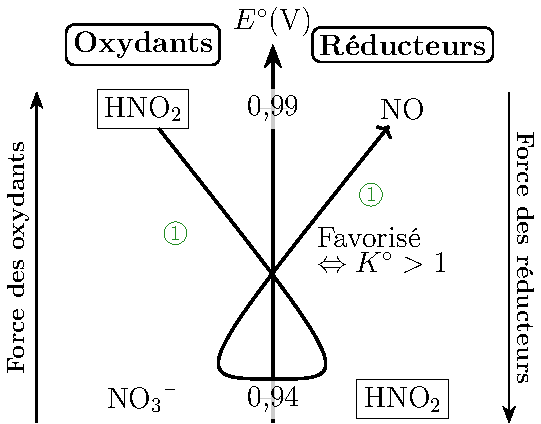
\includegraphics[width=\linewidth]{estand_dismut-hno2}
			% \captionof*{figure}{\protect\pt{1}}
		\end{center}
	\end{minipage}

	% \vspace{0.5cm}%
	% \emph{Autre méthode~:}%
	%
	% En traçant les diagrammes de prédominance des espèces~:
	% \begin{minipage}{0.7\linewidth}%
	% 	On écrit la formule de Nernst pour le couple relatif à la première équation
	% 	:
	%
	% 	$E_1 = E_1^\circ + \cfrac{0,06}{2} \log{\left(
	% 			\cfrac{[\ce{NO3^-}][\ce{H+}]^3}{[\ce{HNO2}](c^\circ)^3} \right)}$ d'où le
	% 	diagramme de prédominance du couple à $\rm pH = 0$ où $E_1 = E_1^\circ$
	%
	% 	De même pour le couple relatif à la deuxième équation~: $E_2 = E_2^\circ +
	% 		\cfrac{0,06}{1} \log{\left( \cfrac{[\ce{HNO2}][\ce{H+}]P^\circ}{(c^\circ)^2
	% 				P_{\ce{NO}}} \right)}$. Or à la frontière~: $\rm pH=0$, $[\ce{HNO_2}]=C_t$
	% 	et $P_{\ce{NO}}=P^\circ$ d'où $E_2 = E_2^\circ$.
	%
	% 	L'espèce $\ce{HNO2}$ est prédominante sur 2 domaines disjoints d'où elle ne
	% 	peut être stable.
	% \end{minipage}%
	% \begin{minipage}{0.27\linewidth}%
	% 	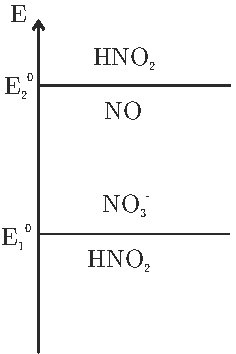
\includegraphics[width=.6\linewidth]{C01}
	% \end{minipage}%
}%

\QR[4]{%
	Donner les degrés d'oxydation de l'azote dans les quatre espèces azotées
	concernées. Établir le diagramme de situation.
}{%
	\label{no}
	\noindent
	\begin{minipage}[t]{.48\linewidth}
		\begin{itemize}
			\item[l][15]{\pt{1}} Dans \ce{NO_{\gaz}}~: $\boxed{\no(\ce{N})=+\myRoman{2}}$
			\item[l][15]{\pt{1}} Dans \ce{HNO2_{\aqu}} et \ce{NO2^-_{\aqu}}~:
			$\boxed{\no(\ce{N})=+\myRoman{3}}$
			\item[l][15]{\pt{1}} Dans \ce{NO3^-_{\aqu}}~: $\boxed{\no(\ce{N})=+\myRoman{5}}$
		\end{itemize}
		On en déduit \xul{le diagramme de situation} \pt{1}~:
	\end{minipage}
	\hfill
	\begin{minipage}[t]{.48\linewidth}
		\vspace{0pt}
		\begin{center}
			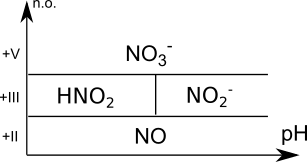
\includegraphics[scale=1]{diag_situation}
		\end{center}
	\end{minipage}
}%


\QR[2]{%
On fournit ci-dessous un diagramme potentiel-pH muet de l'élément azote.
Indiquer la correspondance entre les espèces chimiques \ce{NO_{\aqu}},
\ce{NO3^-_{\aqu}} et \ce{NO2^-_{\aqu}} et les zones I, II et III.
\begin{center}
	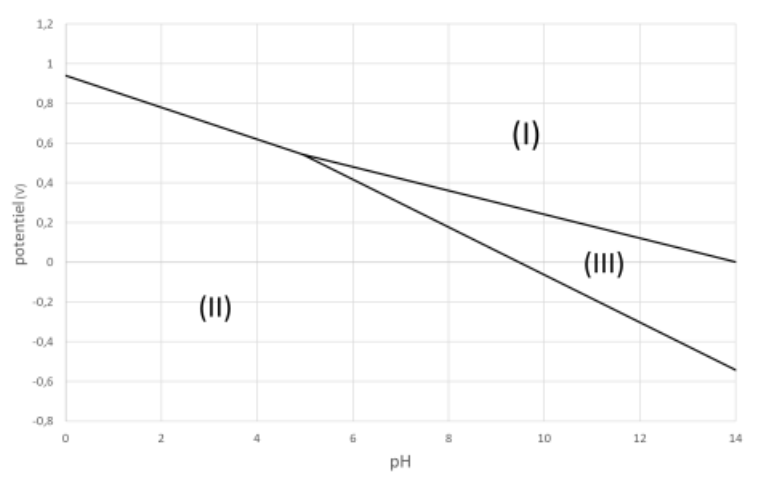
\includegraphics[width=.8\linewidth]{E-pH}
\end{center}
}{%
En réutilisant les résultats de la question \ref{no}, on obtient~:
\begin{tasks}[label=\bdmd](3)
	\task (I)~: Ion nitrate \ce{NO3^-}~;
	\task (II)~: Monoxyde d'azote \ce{NO}~;
	\task (III)~: Ion nitrite \ce{NO2^-}.
\end{tasks}
}%

\QR[4]{%
	Donner l'équation de la frontière entre les domaines I et III. Déterminer le
	potentiel standard du couple redox considéré.
}{%
	\leavevmode\vspace*{-15pt}\relax
	\begin{gather*}
		\ce{{NO_3}^-_{\aqu}} + 2\ce{H^+_{\aqu}} + 2e^- \stm{=}
		\ce{{NO_2}^-_{\aqu}} + \ce{H2O_{\liq}}
		\\\Ra
		E \stm{=}
		E^\circ (\ce{NO3^-}/\ce{NO2^-}) + \frac{0,06}{2}
		\log ( \dfrac{[\ce{NO3^-}][\ce{H^+}]^2}{[\ce{NO2^-}] (c^\circ)^2} )
		\\\beforetext{$[\ce{NO3^-}]\ind{front}=[\ce{NO2^-}]\ind{front}=C_t$}
		\Ra
		\boxed{E\ind{front} \stm{=}
			E^\circ (\ce{NO3^-}/\ce{NO2^-}) - 0,06\pH}%
	\end{gather*}
	La frontière est une \xul{droite de pente -0,06V par unité de pH}.

	Sur le graphique, on lit les coordonnées d'un point par lequel passe cette
	droite frontière~: $\left(\pH=8,0~; E=\SI{0.34}{\volt} \right)$. On calcule alors~:
	\[
		\xul{E^\circ(\ce{NO3^-}/\ce{NO2^-}) \stm{=} \SI{0,82}{\volt}}%
	\]
}%

\subsection{$\mathllap{\textcolor{Red}{/23}\hspace*{1.5cm}}$Teneur en élément azote d'un engrais}

\enonce{%
L'ammonitrate est un engrais azoté solide, bon marché, très utilisé  dans
l'agriculture. Il est vendu par sac de \SI{500}{kg} et contient du nitrate
d'ammonium \ce{NH4NO3_{\sol}}. Les indications fournies par le  fabricant
d'engrais sur le sac à la vente stipulent que le  pourcentage en masse de
\textbf{l'élément azote N} est de 34,4\%.
\bigbreak
Afin de vérifier l'indication du fabricant, on dose les ions ammonium
$\ce{{NH4}^+_{\aqu}}$ présents dans l'engrais en introduisant dans un bécher
$V_1 = \SI{10,0}{\milli \liter}$ d'une solution préparée en dissolvant 6,00 g
d'engrais dans une fiole jaugée de $V_0 = \SI{250}{\milli \liter}$. Cette
solution est dosée à l'aide d'une solution d'hydroxyde de sodium \ce{NaOH} de
concentration $c = \SI{0,200}{\mol \per \liter}$. A l'équivalence, le volume
de soude ajouté $V_E$ est de \SI{14,0}{\milli \liter}.
}%

\QR[2]{%
	Le nitrate d'ammonium est très soluble dans l'eau. Écrire la réaction de
	dissolution correspondante.
}{%
	\leavevmode\vspace*{-15pt}\relax
	\begin{gather*}
		\beforetext{Dissolution du nitrate d'ammonium~:}
		\boxed{\ce{NH4NO3_{\sol} \stm{\stm(un){=}} {NH_4}^+_{\aqu} + {NO_3}^-_{\aqu} }}
	\end{gather*}
}%

\QR[2]{%
L'ion ammonium $\ce{{NH_4}^+_{\aqu}}$ est-il un acide ou une base selon
Brönsted~? Justifier la réponse.
}{%
L'ion ammonium est un acide. \pt{1} C'est \xul{l'acide conjugué de l'ammoniac
	\ce{NH3}}~: il cède un proton. \pt{1}
}%

\QR[2]{%
	Écrire l'équation de la réaction correspondant au titrage.
}{%
	\leavevmode\vspace*{-15pt}\relax
	\begin{gather*}
		\beforetext{Équation de la réaction de titrage~:}
		\boxed{\ce{{NH_4}^+_{\aqu} + HO^-_{\aqu} \stm{\stm(un){=}} NH3_{\aqu} + H2O_{\liq}}}
	\end{gather*}
}%

\QR[3]{%
	La figure ci-après représente la courbe $\pH = f(V_{\text{NaOH}})$. Indiquer
	une méthode graphique pour trouver le point d'équivalence. Donner les
	coordonnées de ce point.
	\begin{center}
		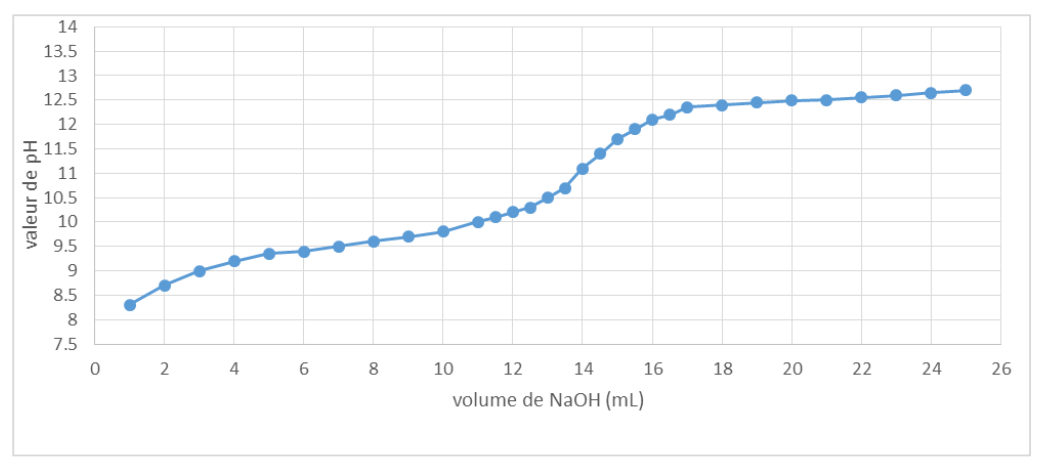
\includegraphics[width=.8\linewidth]{titrage_pH}
	\end{center}
}{%
	En utilisant la méthode des tangentes \pt{1}, on obtient~:
	\[
		\boxed{
			V_E \stm{=} \SI{14,2}{\milli \liter}
			\quad ; \quad
			\pH_E \stm{=} 11,2
		}%
	\]
}%

\QR[3]{%
	Quelles sont toutes les espèces chimiques présentes dans le mélange
	réactionnel à l'équivalence~? Justifier le pH basique de la solution en ce
	point.
}{%
	À l'équivalence, les réactifs ont été consommés \pt{1}, la solution contient
	des ions nitrate et des ions sodium (espèces spectatrices), de l'eau
	(solvant) \pt{1} et de \xul{l'ammoniac \ce{NH3_{\aqu}}} qui est une
	\xul{base faible} \pt{1}, ce qui explique le pH basique.
}%

\QR[4]{%
Donner l'expression littérale de la quantité de matière d'ions
$\ce{{NH_4}^+_{\aqu}}$ dans la fiole jaugée en fonction des données. En
déduire la quantité de nitrate d'ammonium présente dans cette fiole.
}{%
À l'équivalence, les réactifs ont été introduits dans les proportions
stœchiométriques \pt{1}~:
\begin{align*}
	n\ind{\ce{NH4^+},dosé} & = n\ind{\ce{HO^-},versé}
	\\\Lra
	C_1 V_1                & \stm{=} c V_E
\end{align*}
en notant $C_1$ la concentration de la solution préparée en dissolvant l'engrais.
\smallbreak
La quantité de matière de nitrate d'ammonium présente dans la fiole jaugée de
volume $V_0$ s'écrit~:
\[
	\boxed{n_{\ce{NH4+}} = C_1 V_0 \stm{=} \dfrac{c V_E V_0}{V_1}}%
	\Ra
	\xul{n_{\ce{NH4+}} \stm{=} \SI{7,00e-2}{\mole}}%
\]
}%

\QR[7]{%
	Calculer la masse d'azote présente dans l'échantillon. Les indications du
	fabricant sont-elles correctes~?
}{%
	Chaque mole de nitrate d'ammonium \ce{NH4NO3_{\sol}} contient deux moles
	d'élément azote. \pt{1}
	\begin{gather*}
		n_{\ce{N},\rm tot} = 2n_{\ce{NH_4^+}}
		\\\Lra
		\boxed{m(N) \stm[-1]{=} 2n_{\ce{NH_4^+}} M(N)}
		\Ra
		\xul{m(N) \stm{=} \SI{1,96}{g}}
		\\\Lra
		\beforetext{$p$ pourcentage massique}
		\boxed{p = \dfrac{m(N)}{m\ind{engrais}} \stm{=} \dfrac{2n_{\ce{NH_4^+}} M(N)}{m\ind{engrais}}}%
		\Ra
		\xul{p = 0,327 \stm{=} 32,7 \%}
	\end{gather*}
	Le résultat obtenu est proche de l'indication du fabricant. \pt{1} Les
	incertitudes de mesure ne sont pas calculées ici, il n'est pas possible de
	conclure sur la compatibilité entre les deux résultats. \pt{1}
}%

\subsection{$\mathllap{\textcolor{Red}{/28}\hspace*{1.5cm}}$Pollution par les nitrates~: dosage indirect des nitrates}%

\enonce{%
Les nitrates ne sont dangereux pour la santé que s'ils sont en trop grande
concentration dans l'eau. L'Organisation Mondiale de la Santé préconise,
pour une personne, de ne pas consommer plus de \SI{3,65}{mg} d'ions nitrate
par kilogramme de masse corporelle et par jour. La législation française
impose donc une teneur inférieure à \SI{50}{\milli \gram \per \liter}
dans les eaux de consommation. Des analyses sont effectuées régulièrement
pour vérifier la potabilité de l'eau, en particulier la teneur en ions
nitrates.

\paragraph*{Principe du dosage} Lors du dosage indirect, on ajoute un excès de
sel de Mohr, de formule \ce{Fe(SO_4)_2(NH4)_2 6H2O_{\sol}} à un volume connu
d'eau. Dans le sel de Mohr, le fer est à l'état d'oxydation +II.
\smallbreak
Les ions \ce{Fe^2+_{\aqu}} en excès sont ensuite dosés par des ions permanganate
\ce{MnO4^-_{\aqu}}. La concentration en nitrate dans l'eau s'en déduit.

\paragraph*{Protocole expérimental du dosage} Pour effectuer ce dosage, on
introduit dans cet ordre, dans un erlenmeyer, $V_0=\SI{50,0}{\milli \liter}$
d'eau, puis \SI{10}{\milli \liter} de solution d'acide sulfurique \ce{H2SO4} à
\SI{5}{\mole \per \liter} et $V_1=\SI{100,0}{\milli \liter}$ d'une solution
aqueuse de sel de Mohr de concentration molaire $c_1 = \SI{1,00}{\milli \mole
		\per \liter}$.
\smallbreak
Après 45 min de chauffage au bain-marie, on dose ensuite les ions
\ce{Fe^2+_{\aqu}} en excès à l'aide d'une solution de permanganate de potassium
\ce{KMnO4} de concentration $c_2 = \SI{3,00e-4}{\mole \per \liter}$. On repère
l'équivalence grâce au changement de couleur du milieu réactionnel, et on trouve
un volume équivalent $V=\SI{11,0}{\milli \liter}$ pour l'eau analysée.
}%

\QR[2]{%
Écrire les deux demi-équations d'oxydo-réduction des couples
$\ce{{NO_3}^-_{\aqu}/NO_{\gaz}}$ et $\ce{Fe^3+_{\aqu}/Fe^2+_{\aqu}}$.
}{%
\leavevmode\vspace*{-15pt}\relax
\begin{align*}
	\beforetext{Couple $\ce{{NO_3}^-_{\aqu}/NO_{\gaz}}$}
	\ce{{NO_3}^-_{\aqu} + 4H^+_{\aqu} + 3e^- & \stm{=} NO_{\gaz} + 2H2O_{\liq}}
	\\\beforetext{Couple $\ce{Fe^3+_{\aqu}/Fe^2+_{\aqu}}$}
	\ce{Fe^3+_{\aqu} + e^-                   & \stm{=} Fe^2+_{\aqu}}
\end{align*}
}%

\QR[12]{%
	En déduire l'équation de la réaction d'oxydo-réduction ayant lieu dans
	l'erlenmeyer avant le dosage. Justifier le fait que cette réaction est
	quasi-totale en déterminant l'expression puis en calculant la constante
	d'équilibre de cette réaction. Quel aspect de la réaction cette constante ne
	traite-t-elle pas~? Pour quelle probable raison fait-on un titrage
	indirect~? Quelle serait une autre raison~?
}{%
	À partir des demi-équations précédentes, on obtient l'équation de la
	réaction~:
	\begin{gather*}
		\ce{NO3^-_{\aqu} + 3Fe^2+_{\aqu} + 4H^+_{\aqu} \stm{\stm(un){=}}
		NO_{\gaz} + 3Fe^3+_{\aqu} + 2H2O_{\liq}}
		\tag*{$\DS K^\circ \stm{=}
			\cfrac{[\ce{Fe^{3+}}]^3 P_{\ce{NO}} (c^\circ)^5}
			{[\ce{NO3^-}] [\ce{Fe^2+}]^3 [\ce{H3O+}]^4 P^\circ}$
		}
	\end{gather*}
	À l'équilibre il y a égalité des potentiels des couples en présence \pt{1}, d'où
	\begin{align*}
		E (\ce{{NO_3}^-_{\aqu}/NO_{\gaz}})
		 & =
		E (\ce{Fe^3+_{\aqu}/Fe^2+_{\aqu}})
		\\\Lra
		E^\circ(\ce{NO3^-}/\ce{NO}) + \cfrac{0,06}{3}
		\log( \cfrac{[\ce{NO3^-}] [\ce{H3O+}]^4 P^\circ}{P_{\ce{NO}} (c^\circ)^5 })
		 & \stm{\stm(un){=}}
		E^\circ ( \ce{Fe^3+} / \ce{Fe^2+} ) + \cfrac{0,06}{1}
		\log( \cfrac{[\ce{Fe^3+}]}{[\ce{Fe^2+}]} )
		\\\Lra
		E^\circ \left( \ce{NO3^-} / \ce{NO} \right) - E^\circ \left( \ce{Fe^3+} /
		\ce{Fe^2+} \right)
		 & = \cfrac{0,06}{3} \log{(K^\circ)}
		\\\Ra
		\Aboxed{K^\circ
		 & \stm{=}
			10^{\DS \frac{3}{\num{0.06}} \left( E^\circ (\ce{{NO_3}^-} / \ce{NO}) -
					E^\circ ( \ce{Fe^3+} / \ce{Fe^2+}) \right)}
		}%
		\\
		\makebox[0pt][l]{$\phantom{\AN}\xul{\phantom{K^\circ = 10^{9,5}}}$}
		\AN
		K^\circ
		 & \stm{=} 10^{9,5}
	\end{align*}
	La constante d'équilibre $K^\circ \gg 10^3$ donc \xul{on peut considérer la
		réaction quasi-totale} \pt{1}. Cependant, elle ne nous renseigne pas sur la
	cinétique \pt{1} de la réaction. On réalise un titrage indirect sans doute
	parce que la réaction est lente \pt{1}. Autrement, le suivi potentiométrique
	est peut-être difficile à suivre, par exemple avec un \textbf{faible saut}
	de potentiel \pt{1}.
}%

\QR[3]{%
	En déduire une relation entre la quantité de matière de \ce{Fe^2+} restant
	présente dans l'erlenmeyer et les quantités de matière initiales des réactifs
	$n\ind{\ce{Fe^2+} initiale}$ et $n\ind{\ce{NO3^-}~initiale}$.
}{%
	\label{mol}Quantité de matière de \ce{Fe^2+} restant présente dans l'erlenmeyer~:
	\begin{align*}
		n\ind{\ce{Fe^2+} restant}         & \stm{=}
		n\ind{\ce{Fe^2+} initiale} - n\ind{\ce{Fe^2+}~ayant~réagi~avec~\ce{NO3^-}}
		\\\Lra
		\beforetext{Avec la stœchiométrie \pt{1}}
		\Aboxed{n\ind{\ce{Fe^2+} restant} & \stm{=}
			n\ind{\ce{Fe^2+}~initiale} - 3 n\ind{\ce{NO3^-}~initiale}}
	\end{align*}
}%

\QR[3]{%
Écrire la réaction du dosage des ions \ce{Fe^2+_{\aqu}} par les ions permanganate.
}{%
\leavevmode\vspace*{-15pt}\relax
\begin{gather*}
	\beforetext{Couple $\ce{{MnO_4}^-_{\aqu}/Mn^2+_{\aqu}}$}
	\ce{{MnO_4}^-_{\aqu} + 8H^+_{\aqu} + 5e^- \stm{=} Mn^2+_{\aqu} + 4H2O_{\liq}}
	\\\beforetext{Titrage}
	\boxed{
	\ce{
	{MnO_4}^-_{\aqu} + 8H^+_{\aqu} + 5Fe^2+_{\aqu} \stm{\stm(un){=}}
	Mn^2+_{\aqu} + 4H2O_{\liq} + 5Fe^3+_{\aqu}
	}
	}
\end{gather*}
}%

\QR[4]{%
Donner l'expression littérale permettant de calculer la quantité d'ions
\ce{NO3^-_{\aqu}} présents dans l'échantillon d'eau. Vérifier qu'on obtient
\SI{2,78e-5}{\mole} d'ions \ce{NO3^-_{\aqu}}.
}{%
\leavevmode\vspace*{-15pt}\relax
\begin{align*}
	\beforetext{D'après la question \ref{mol}, nous avons~:}
	n\ind{\ce{NO3^-}~initiale} & =
	\frac{1}{3} ( n\ind{\ce{Fe^2+}~initiale} - n\ind{\ce{Fe^2+} restant} )
	\shortintertext{À l'équivalence du titrage, les réactifs ont été introduits
		dans les proportions stœchiométriques~:}
	n\ind{\ce{Fe^2+} titré}    & \stm{=}
	5 n\ind{\ce{MnO4^-}~versé}
	\\\Lra
	n\ind{\ce{Fe^2+} restant}  & = 5 c_2 V
	\\\beforetext{Or,}
	n\ind{\ce{Fe^2+}~initiale} & = c_1 V_1
	\\\Ra
	\Aboxed{
	n\ind{\ce{NO3^-}~initiale} & \stm{=}
		\frac{1}{3} \left( c_1 V_1 - 5c_2 V \right)
	}
	\\
	\makebox[0pt][l]{$\phantom{\AN}\xul{\phantom{n\ind{\ce{NO3^-}~initiale} = \SI{2,78e-5}{\mole}}}$}
	\AN
	n\ind{\ce{NO3^-}~initiale} \stm{=} \SI{2,78e-5}{\mole}
\end{align*}
ce qui correspond à la valeur fournie par l'énoncé \pt{1}.
}%

\QR[3]{%
	Peut-on considérer que l'eau dosée soit considérée comme potable~?
}{%
	\leavevmode\vspace*{-15pt}\relax
	\begin{gather*}
		\beforetext{Concentration massique en ions nitrate~:}
		\boxed{C_m \stm{=} \dfrac{n\ind{\ce{NO3^-}~initiale} M(\ce{NO3^-})}{V_0}}
		\\\AN
		\xul{C_m = \SI{3,45e-2}{g.L^{-1}} \stm{=} \SI{34,5}{mg.L^{-1}}}
	\end{gather*}
	La valeur obtenue est inférieure à la teneur maximale autorisée
	(\SI{50}{mg.L^{-1}})~: cette eau est \xul{potable}. \pt{1}
}%

\QR[4]{%
	Quel volume de cette eau um enfant de \SI{35}{kg} peut-iel boire par jour sans
	préjudices pour sa santé~? Commenter.
}{%
	La masse maximale d'ions nitrate que peut consommer cæt enfant de masse $m$
	égale à \SI{35}{kg} est~:
	\begin{gather*}
		m\ind{nitrates max} \stm{=} x \times m
		\qav
		x = \SI{3,65}{\milli \gram \per \kilo \gram}
	\end{gather*}
	Cherchons le volume $V\ind{eau}$ qui contient cette masse~:
	\begin{gather*}
		\boxed{V\ind{eau} \stm{=} \dfrac{m\ind{nitrates max}}{C_m}}
		\\\AN
		\xul{V\ind{eau} \stm{=} \SI{3,70}{\liter}}
	\end{gather*}
	Avec une concentration massique de \SI{50}{\milli \gram \per \liter} (limite
	autorisée), l'application numérique donne \SI{2,6}{\liter}, ce qui est sans
	doute supérieur \pt{1} au volume d'eau consommé par um enfant en une journée.
}%

\end{document}%
